\chapter{Założenia projektowe}
\label{chap:zalozenia-projektowe}
\section{Wymagania funkcjonalne}
\label{sec:wymagania-funkcjonalne}

W tej sekcji opisane zostaną wymagania funkcjonalne jakie powinien spełniać stworzony system. Zaprezentowane zostaną przypadki użycia dla czterech podsystemów: system zarządzania kontem pieniężnym, system zarządzania środkami finansowymi, system zarządzania rodziną i system zarządzania kategoriami. Przypadki użycia zostaną opisane w schemacie: nazwa przypadku użycia, aktor wykonujący akcję, warunki początkowe, warunki końcowe, cel oraz przebieg. Ponadto przypadki użycia zostaną zaprezentowane w formie diagramów.

\subsection{Wymagania dotyczące konta pieniężnego}
\label{subsec:wymagania-konto}
Poniżej opisano przypadki użycia dotyczące zarządzania kontem pieniężnym użytkownika. Zaprezentowano je także na diagramie (rys.~\ref{fig:use-case-account}).

\begin{enumerate}[labelwidth=1em,label=\arabic*.]
\item \textbf{Nazwa:} Dodaj konto \newline
    \textbf{Aktor:} Zalogowany użytkownik \newline
    \textbf{Warunki początkowe:} Użytkownik musi się wcześniej zarejestrować i być zalogowany w momencie tworzenia konta. \newline
    \textbf{Warunki końcowe:} Stan konta musi być zgodny z polityką dla jego typu. \newline
    \textbf{Cel:} Stworzenie w systemie konta pieniężnego przypisanego do aktora wykonującego tę operację, aby umożliwić zapisywanie informacji o przepływie gotówki. \newline
    \textbf{Przebieg:} Użytkownik wypełnia formularz. Wpisuje wymagane pola: nazwa konta, saldo początkowe i limit debetu oraz opcjonalne pola: numer konta, waluta i opis. Wybiera także typ konta.
\item \textbf{Nazwa:} Usuń konto \newline
    \textbf{Aktor:} Właściciel konta \newline
    \textbf{Warunki początkowe:} Użytkownik musi posiadać konto pieniężne. \newline
    \textbf{Warunki końcowe:} Użytkownik musi potwierdzić usunięcie konta. \newline
    \textbf{Cel:} Usunięcie konta pieniężnego użytkownika wraz z jego historią. \newline
    \textbf{Przebieg:} Użytkownik wybiera jedno ze swoich kont, a następnie naciska guzik usuń. Użytkownik musi potwierdzić tę operację.
\item \textbf{Nazwa:} Edytuj dane konta \newline
    \textbf{Aktor:} Właściciel konta \newline
    \textbf{Warunki początkowe:} Użytkownik musi posiadać konto pieniężne. \newline
    \textbf{Warunki końcowe:} Stan konta nie może przekraczać nowego limitu debetu. \newline
    \textbf{Cel:} Aktualizacja danych konta, bez utraty jego historii. \newline
    \textbf{Przebieg:} Użytkownik edytuje pola obowiązkowe formularza: nazwa konta, limit debetu oraz opcjonalne pola: numer konta, waluta i opis. Nie może edytować jego typu.
\item \label{last-item1}\textbf{Nazwa:} Zmień typ konta\newline
    \textbf{Aktor:} Właściciel konta \newline
    \textbf{Warunki początkowe:} Użytkownik musi posiadać konto pieniężne. \newline
    \textbf{Warunki końcowe:} Typ konta musi pozwalać na potencjalnie istniejący na koncie debet. \newline
    \textbf{Cel:} Zmiana typu konta na inny. Umożliwiające posiadanie debetu, lub oprocentowane. \newline
    \textbf{Przebieg:} Użytkownik po wybraniu konta zmienia jego typ, a swój wybór zatwierdza naciśnięciem guzika ,,Akceptuj''. 
\end{enumerate}

\begin{figure}[t]
	\centering
	\fbox{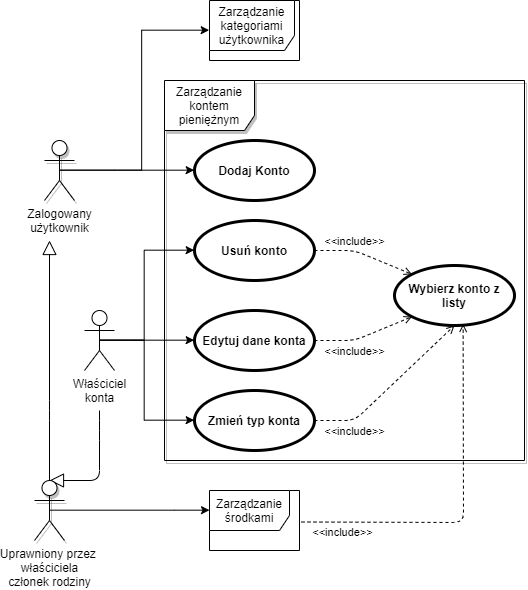
\includegraphics[width=.65\linewidth]{rys03/use-case-account.png}}
	\caption{Diagram przypadków użycia konta pieniężnego}
	\label{fig:use-case-account}
\end{figure}

\subsection{Wymagania dotyczące środków finansowych}
\label{subsec:wymagania-srodki-finansowe}
Na rysunku~\ref{fig:use-case-money} przedstawiono przypadki użycia związane z definiowaniem przepływu gotówki dla kont pieniężnych. Poniżej znajdują się także ich opisy.

\begin{enumerate}[labelwidth=1em,label=\arabic*.]
\item \textbf{Nazwa:} Dodaj wydatek/przychód \newline
    \textbf{Aktor:} Uprawniony przez właściciela członek rodziny \newline
    \textbf{Warunki początkowe:} Administrator rodziny zdefiniował co najmniej jedną kategorię dla operacji finansowych. \newline
    \textbf{Warunki końcowe:} Stan konta po operacji dodania wydatku musi być zgodny z polityką dla typu konta. \newline
    \textbf{Cel:} Zdefiniowanie operacji pieniężnej w ramach konta. \newline
    \textbf{Przebieg:} Użytkownik tworzy wydatek lub przychód wpisując obowiązkowe pola: kwota i data, a także te dodatkowe: notatka, odbiorca. Użytkownik musi także wybrać kategorię. 
\item \textbf{Nazwa:} Usuń wydatek/przychód \newline
    \textbf{Aktor:} Uprawniony przez właściciela członek rodziny \newline
    \textbf{Warunki początkowe:} Konto posiada co najmniej jeden wpis: wydatek lub przychód. \newline
    \textbf{Warunki końcowe:} Stan konta po operacji usunięcia przychodu musi być zgodny z polityką dla typu konta. \newline
    \textbf{Cel:} Usunięcie operacji pieniężnej w ramach konta. \newline
    \textbf{Przebieg:} Użytkownik wybiera wydatek lub przychód, a następnie naciska guzik usuń. 
\item \textbf{Nazwa:} Edytuj wydatek/przychód \newline
    \textbf{Aktor:} Uprawniony przez właściciela członek rodziny \newline
    \textbf{Warunki początkowe:} Konto posiada co najmniej jeden wpis: wydatek lub przychód. \newline
    \textbf{Warunki końcowe:} Stan konta po edycji wpisu musi być zgodny z polityką dla typu konta. \newline
    \textbf{Cel:} Edycja operacji pieniężnej w ramach konta. \newline
    \textbf{Przebieg:} Użytkownik wybiera wydatek lub przychód, a następnie naciska guzik ,,edytuj''. Edytuje pola obowiązkowe i dodatkowe. Jeśli chce zmienić kategorię musi ją wybrać z listy. \newline
    \textbf{Rozszerzenia: } 
    \begin{enumerate}[label=\alph*)]
        \item Użytkownik edytuje kategorię wpisu: Wybór kategorii.
    \end{enumerate}
\item \textbf{Nazwa:} Wykonaj przelew \newline
    \textbf{Aktor:} Uprawniony przez właściciela członek rodziny \newline
    \textbf{Warunki początkowe:} Administrator rodziny zdefiniował co najmniej jedną kategorię dla operacji finansowych. \newline
    \textbf{Warunki końcowe:} Stan konta po przelewie musi być zgodny z polityką dla typu konta. \newline
    \textbf{Cel:} Wykonanie przelewu między kontami lub zewnętrznego. \newline
    \textbf{Przebieg:} Użytkownik definiuje przelew wpisując obowiązkowe pola: kwota i data, a także dodatkowe: notatka, odbiorca. Użytkownik musi także wybrać kategorię. \newline
    \textbf{Rozszerzenia: }
    \begin{enumerate}[label=\alph*)]
        \item Użytkownik definiuje przelew między kontami rodziny: Przelew własny.
    \end{enumerate}
\end{enumerate}

\begin{figure}[t]
	\centering
	\fbox{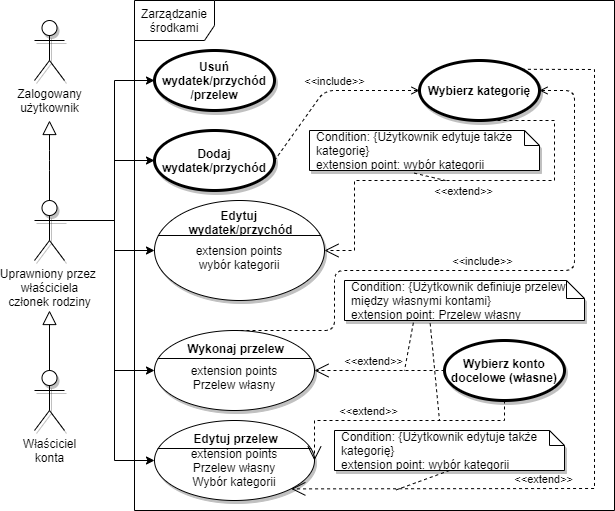
\includegraphics[width=.7\linewidth]{rys03/use-case-money.png}}
	\caption{Subdiagram przypadków użycia dla operacji finansowych}
	\label{fig:use-case-money}
\end{figure}

\subsection{Wymagania dotyczące rodziny}
\label{subsec:wymagania-rodzina}
Wymagania funkcjonalne dotyczące obsługi w aplikacji grupy rodziny, dalej zwanej rodziną, przedstawione zostały na~ rysunku~\ref{fig:use-case-family}. Poniżej znajdują się także ich szczegółowe opisy.

\begin{enumerate}[labelwidth=1em,label=\arabic*.]
\item \textbf{Nazwa:} Stwórz rodzinę \newline
    \textbf{Aktor:} Zalogowany użytkownik \newline
    \textbf{Warunki początkowe:} Użytkownik zarejestrował się w aplikacji. \newline
    \textbf{Warunki końcowe:} Użytkownik staje się administratorem nowoutworzonej rodziny. \newline
    \textbf{Cel:} Stworzenie rodziny, w ramach której można współdzielić konta pieniężne i ich historie. \newline
    \textbf{Przebieg:} Rodzina zostaje stworzona w momencie rejestracji. 
\item \textbf{Nazwa:} Akceptuj zaproszenie \newline
    \textbf{Aktor:} Zalogowany użytkownik \newline
    \textbf{Warunki początkowe:} Administrator innej rodziny dodał do niej użytkownika. \newline
    \textbf{Warunki końcowe:} Użytkownik zaakceptował zaproszenie.  \newline
    \textbf{Cel:} Dołączenie do nowej rodziny. \newline
    \textbf{Przebieg:} Użytkownik wyświetla zaproszenia do rodziny. Następnie akceptuje zaproszenie do jednej, bądź wielu z nich.
\item \textbf{Nazwa:} Dodaj członka \newline
    \textbf{Aktor:} Administrator rodziny \newline
    \textbf{Warunki początkowe:} Użytkownik stworzył rodzinę. \newline
    \textbf{Warunki końcowe:} Użytkownik akceptuje zaproszenie do rodziny.  \newline
    \textbf{Cel:} Dodanie nowego członka do rodziny, aby współdzielić historię finansową. \newline
    \textbf{Przebieg:} Administrator wpisuję login użytkownika, którego chce dodać i zatwierdza wybór guzikiem. 
\item \textbf{Nazwa:} Usuń członka \newline
    \textbf{Aktor:} Administrator rodziny \newline
    \textbf{Warunki początkowe:} Użytkownik dodał do rodziny co~najmniej jednego innego członka. \newline
    \textbf{Warunki końcowe:} --  \newline
    \textbf{Cel:} Usunięcie członka z rodziny. \newline
    \textbf{Przebieg:} Administrator naciska guzik usuń członka, a następnie potwierdza swoją akcję.
\item \textbf{Nazwa:} Edytuj uprawnienia dostępu do konta \newline
    \textbf{Aktor:} Członek rodziny będący właścicielem konta \newline
    \textbf{Warunki początkowe:} Użytkownik jest właścicielem konta. W rodzinie, do której przypisane jest konto jest więcej niż jeden członek. \newline
    \textbf{Warunki końcowe:} Właściciel konta potwierdza nadanie uprawnień naciskając guzik. \newline
    \textbf{Cel:} Nadanie uprawnień członkowi rodziny, aby mógł publikować wpisy w ramach konta i/lub przeglądać jego historię.  \newline
    \textbf{Przebieg:} Właściciel konta wybiera z listy jedno ze swoich kont w ramach rodziny. Następnie z listy wybiera członka rodziny, któremu chce nadać uprawnienia. Nadaje członkowi uprawnienia spośród: prawo do wglądu, prawo do dodawania wpisów.
    Swój wybór zatwierdza guzikiem ,,zatwierdź''.
\end{enumerate}

\begin{figure}[t]
	\centering
	\fbox{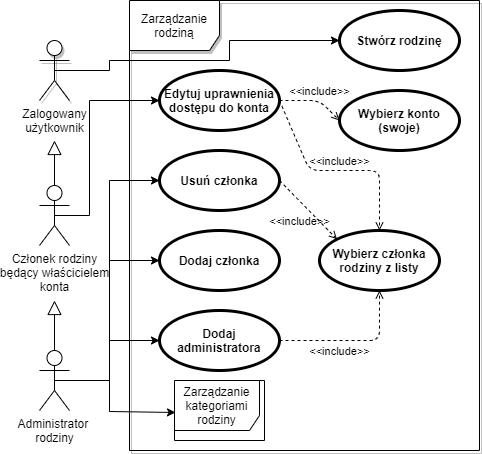
\includegraphics[width=.65\linewidth]{rys03/use-case-family.png}}
	\caption{Diagram przypadków użycia dla rodziny}
	\label{fig:use-case-family}
\end{figure}

\subsection{Wymagania dotyczące kategorii}
\label{subsec:wymagania-kategorie}

\begin{enumerate}[labelwidth=1em,label=\arabic*.]
\item \textbf{Nazwa:} Dodaj kategorię \newline
    \textbf{Aktor:} Zalogowany użytkownik \newline
    \textbf{Warunki początkowe:} Użytkownik zarejestrował się w aplikacji. \newline
    \textbf{Warunki końcowe:} Nazwa kategorii w swoim poddrzewie jest unikatowa. \newline
    \textbf{Cel:} Stworzenie kategorii, aby łatwiej segregować wydatki i przychody. \newline
    \textbf{Przebieg:} Użytkownik naciska guzik dodaj kategorię na drzewie kategorii. Następnie wpisuje jej nazwę i wybiera kolor wyświetlania wpisów przypisanych do niej.
\item \textbf{Nazwa:} Edytuj kategorię \newline
    \textbf{Aktor:} Zalogowany użytkownik \newline
    \textbf{Warunki początkowe:} Użytkownik dodał co najmniej jedną kategorię. \newline
    \textbf{Warunki końcowe:} Nazwa kategorii w swoim poddrzewie jest unikatowa. \newline
    \textbf{Cel:} Edycja istniejącej kategorii bez utraty historii wpisów tej kategorii. \newline
    \textbf{Przebieg:} Użytkownik edytuje nazwę i kolor kategorii. Może także przeciągnąć ją do innej kategorii nadrzędnej lub zrobić z niej kategorię najwyższego rzędu.
\item \textbf{Nazwa:} Ukryj kategorię \newline
    \textbf{Aktor:} Zalogowany użytkownik \newline
    \textbf{Warunki początkowe:} Użytkownik dodał co najmniej jedną kategorię. \newline
    \textbf{Warunki końcowe:} -- \newline
    \textbf{Cel:} Ukrycie istniejącej kategorii bez utraty historii wpisów tej kategorii. \newline
    \textbf{Przebieg:} Użytkownik w menu kategorii klika ukryj.
\item \textbf{Nazwa:} Usuń kategorię \newline
    \textbf{Aktor:} Zalogowany użytkownik \newline
    \textbf{Warunki początkowe:} Użytkownik dodał co najmniej jedną kategorię. Kategoria nie posiada żadnych wpisów. \newline
    \textbf{Warunki końcowe:} Nie istnieje wpis, który nie ma przypisanej kategorii. \newline
    \textbf{Cel:} Usunięcie kategorii, do której nie jest przypisany żaden wpis. \newline
    \textbf{Przebieg:} Użytkownik w menu kategorii klika usuń i zatwierdza wybór.
\end{enumerate}

\begin{figure}[t]
	\centering
	\fbox{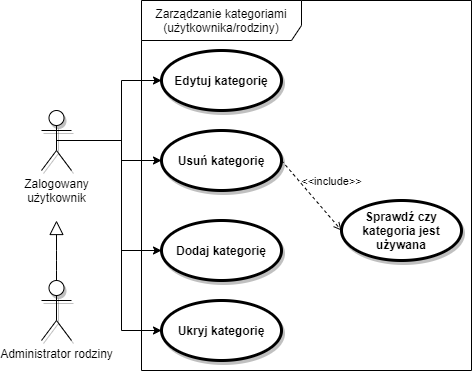
\includegraphics[width=.65\linewidth]{rys03/use-case-category.png}}
	\caption{Diagram przypadków użycia dla kategorii}
	\label{fig:use-case-category}
\end{figure}

\section{Wymagania niefunkcjonalne}
\label{sec:wymagania-niefunkcjonalne}

\begin{enumerate}[labelwidth=1em,label=\arabic*.]

\item System składać ma się z~dwóch głównych części:
\begin{enumerate}[label=\alph*)]
\item aplikacji serwerowej -- API. Jej zadaniem będzie dostarczanie interfejsu programistycznego do pobierania danych i~modyfikowania stanu systemu.
\item aplikacja webowej, dostarczająca graficzny interfejs użytkownika -- \texttt{GUI}. Aplikacja ta będzie konsumować API.
\end{enumerate}

\item Zarówno aplikacja webowa, jak i API będą stworzone przy pomocy frameworka ASP.NET Core w wersji co najmniej 2.2: 
\begin{enumerate}[label=\alph*)]
\item Do napisania aplikacji webowej użyte zostaną \texttt{Razor Pages} oraz komponenty widoku (ang.~\emph{view components}). 
\item Warstwa persystencji danych w aplikacji API stworzona zostanie z pomocą Entity Framework Core 2.2. Wykorzystane zostanie podejście \emph{code first} i mechanizm migracji.
\end{enumerate}

\item Pobieranie danych z API ma odbywać się za pomocą protokołu OData.

\item API używać będzie bazy danych na serwerze Microsoft SQL Server 2017 (lub nowszym).

\item Aplikacja webowa powinna poprawnie działać co najmniej w przeglądarkach: Mozilla Firefox, Google Chrome, Opera, Microsoft Edge oraz Safari, a~także przeglądarkach mobilnych: Opera Mobile, Google Chrome, Mozilla Firefox i Safari.

\item Aplikacja będzie wymuszać działanie z wykorzystaniem protokołu \texttt{HTTPS} (ang.~\emph{Hypertext Transfer Protocol Secure}).

\item Autoryzacja i uwierzytelnienie ma być przeprowadzona z wykorzystaniem protokołu OpenId Connect i frameworka autoryzacji OAuth 2.0. Użyty powinien zostać \emph{Hybrid Flow} lub \emph{Authorization Code Flow}.

\item Dostawcą tożsamości w systemie powinna być osobna aplikacja, posiadająca własną bazę danych lub zewnętrzy system autoryzacji, np.~\texttt{Auth0}.

\item API ma posiadać dokumentację stworzoną przy pomocy narzędzia \texttt{Swagger}.

\item Kod źródłowy ma być napisany z wykorzystaniem dobrych praktyk programowania~i~wzorców projektowych ułatwiających jego utrzymanie i rozwijanie.

\item System działać będzie na platformie chmurowej \texttt{Microsfot Azure}.

\item Poszczególne składowe systemu w chmurze powinny być automatycznie skalowalne.

\item Aplikacja webowa powinna być bezpieczna i odporna na ataki. Zostanie wykorzystany mechanizm obrony przed \texttt{CSRF} (ang.~Cross-Site Request Forgery) -- \texttt{anti-forgery token}.

\end{enumerate}

\section{Metodyka}
\label{sec:metodyka}